\subsection{GameGUI}
GUI klassen er det grafiske. Her kan vi vise en bil i en bestemt farve som spilleren er blvet tildelt. Der oprettes altså spillere. Dette ses på følgende billede:

\begin{figure}[H]
    \centering
    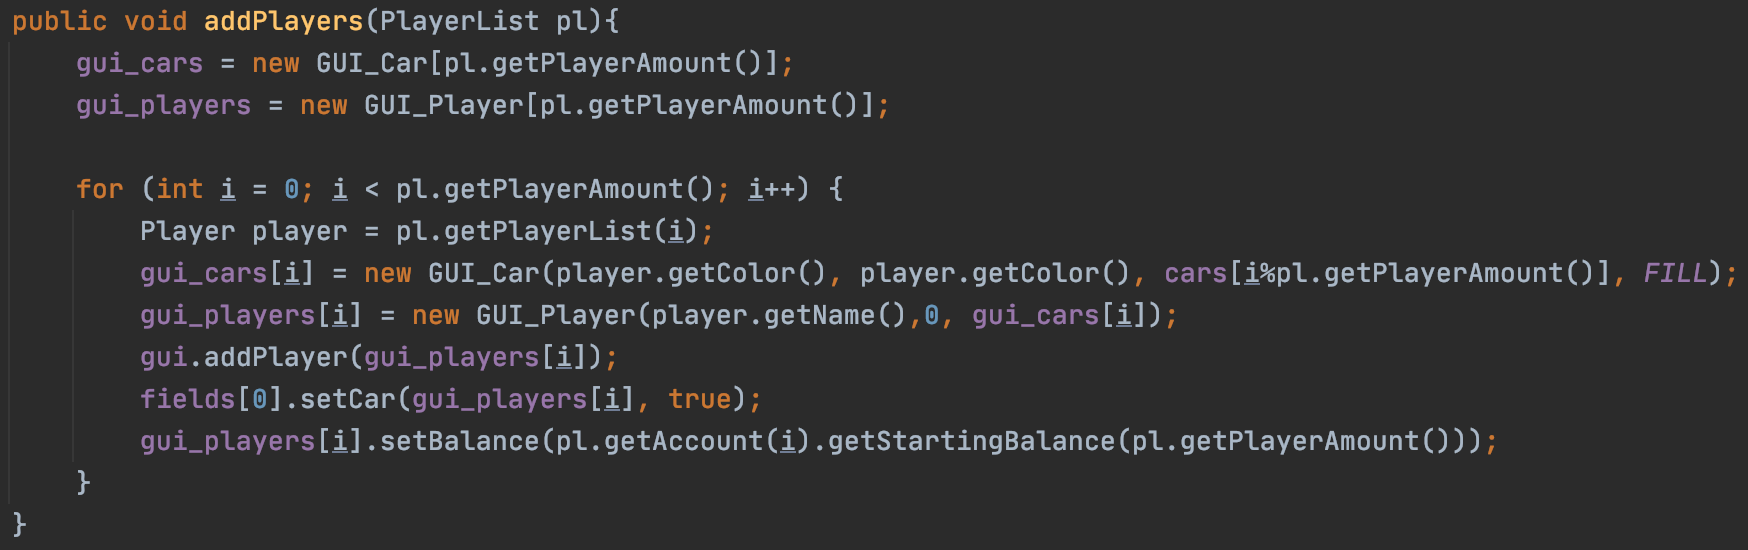
\includegraphics[width=0.7\textwidth]{sources/7_implementering/GameGUIaddPlayers.png}
    \caption{Bil \& farve tildeles spillerne}
    \label{fig:playerListklasse}
\end{figure}

GameGUI klassen skal bruge en konstuktør. Derfor oprettes følgende konstuktør for vores GUI:
\begin{figure}[H]
    \centering
    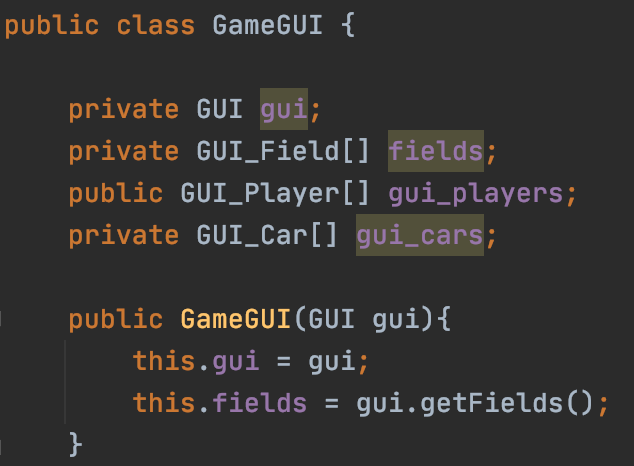
\includegraphics{sources/7_implementering/GameGUIclass.png}
    \caption{Konstruktør}
    \label{fig:playerListklasse}
\end{figure}

Når en spiller lander på et chance-kort, så skal kortet med teksten vises til spillerne. Det er gjort ved at kalde på den beske, som er tilknyttet chancekortet, så teksten kan sættes på et "fysisk" chance-kort:
\begin{figure}[H]
    \centering
    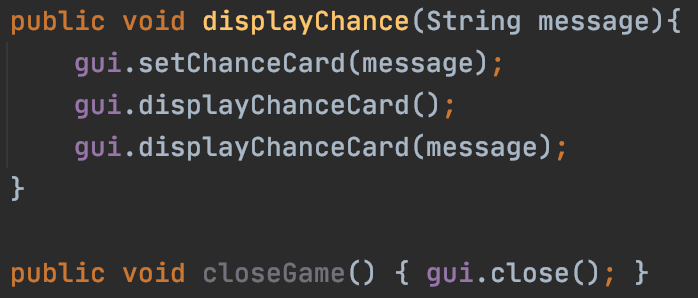
\includegraphics{sources/7_implementering/GameGUIdisplayChance.png}
    \caption{Chance-kort besked}
    \label{fig:playerListklasse}
\end{figure}

Metoden "fancyMoveGuiPlayer" og "moveToField" Rykker spillernes brikker med rundt på spillepladen. Dette kan ses på de følgende to billeder: 
\begin{figure}[H]
    \centering
    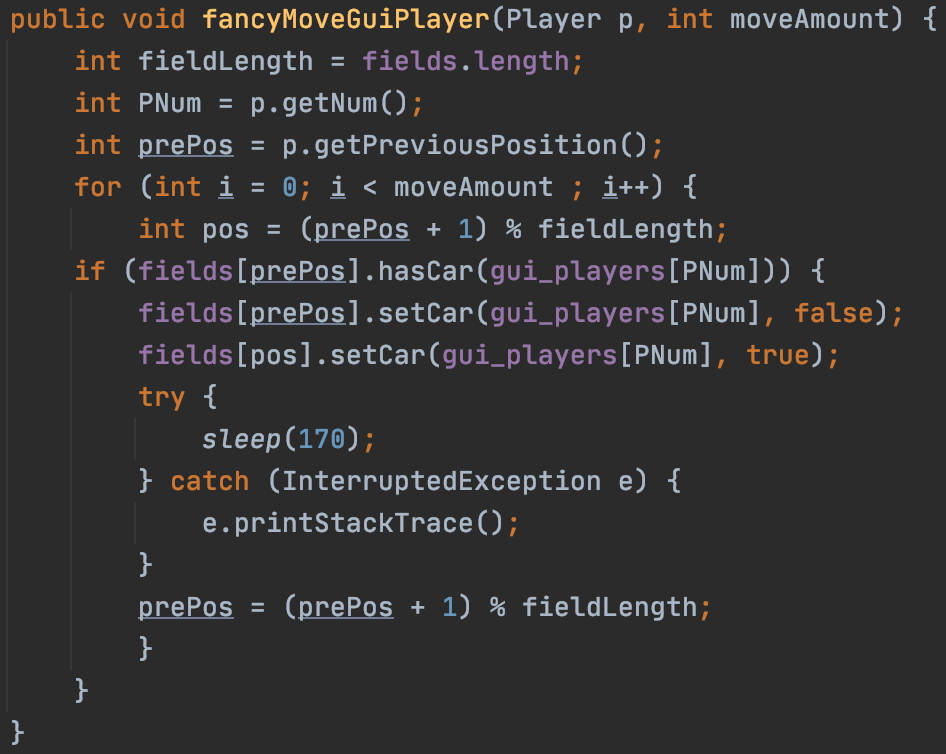
\includegraphics{sources/7_implementering/GameGUIfancyMove.png}
    \caption{fancyMoveGuiPlayer-klassen}
    \label{fig:GUIklasse}
\end{figure}
moveToField sørger for, at brikken rykker sig til en ny position på spilbrættet.
\begin{figure}[H]
    \centering
    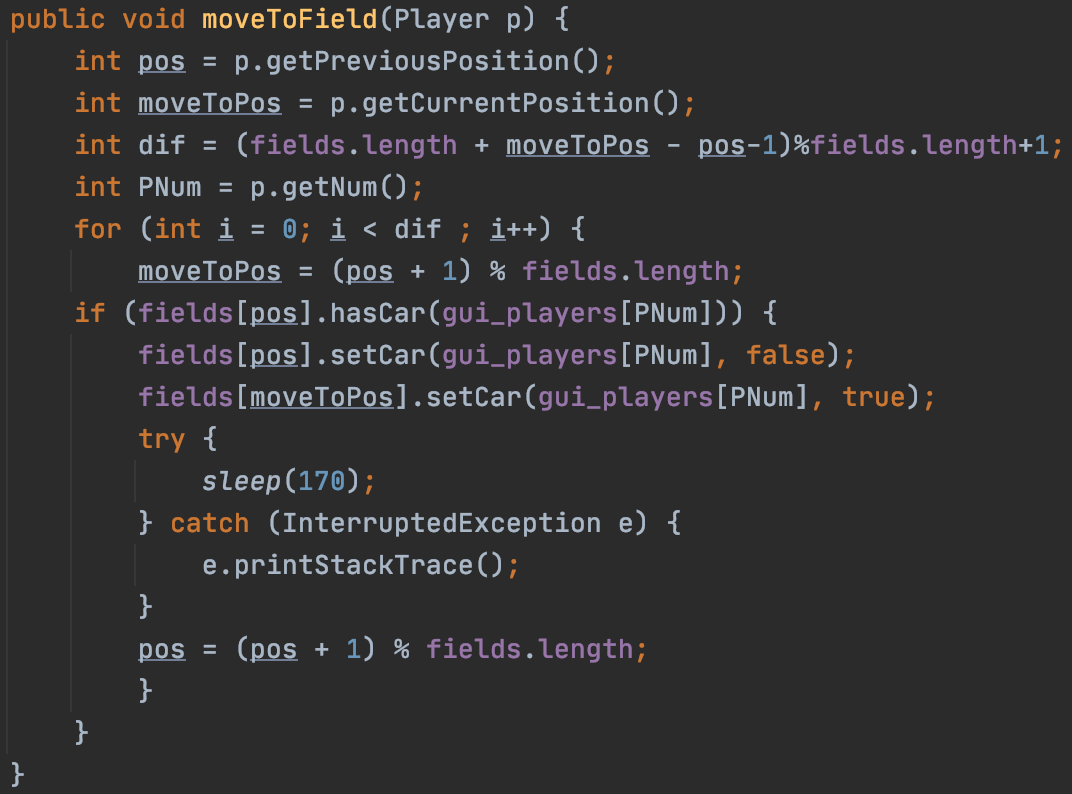
\includegraphics[width=0.7\textwidth]{sources/7_implementering/GameGUImoveToField.png}
    \caption{moveToField-klassen}
    \label{fig:GUImoveToField}
\end{figure}
"showBalance" viser spillerne hvor mange penge de har:
\begin{figure}[H]
    \centering
    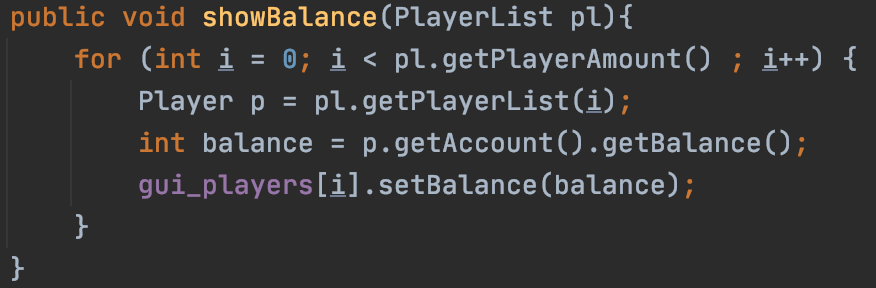
\includegraphics{sources/7_implementering/GameGUIshowBalance.png}
    \caption{Balance}
    \label{fig:GUIbalance}
\end{figure}
Når spilleren slår med terningen, så viser denne metode de visuelle kast/resultat:
\begin{figure}[H]
    \centering
    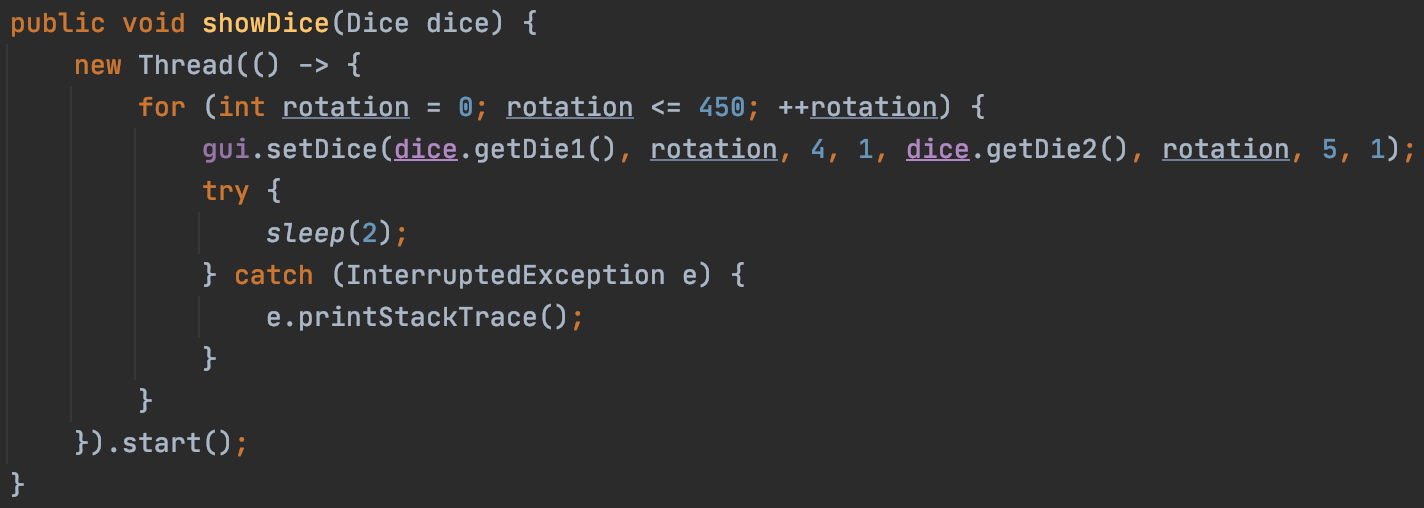
\includegraphics[width=0.7\textwidth]{sources/7_implementering/GameGUIshowDice.png}
    \caption{Terning}
    \label{fig:GUIterning}
\end{figure}
Metoden "showMessage" viser beskederne, som f.eks. spørger spilleren om man vil slå med terningen, købe grunden eller andre lignende beskeder:
\begin{figure}[H]
    \centering
    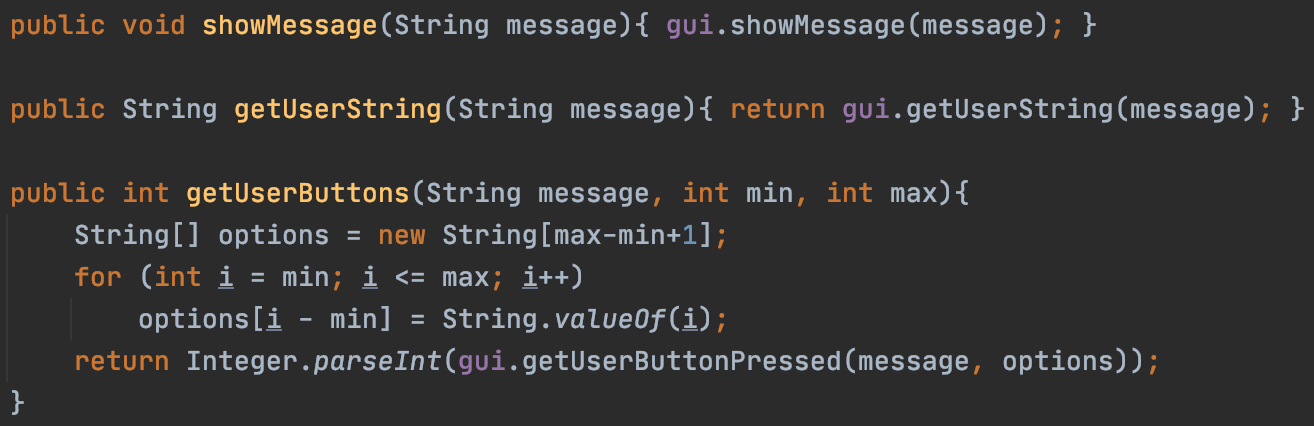
\includegraphics{sources/7_implementering/GameGUIshowMessage.png}
    \caption{Beskeder}
    \label{fig:GUIbeskeder}
\end{figure}
Når et felt bliver købt, så bliver feltet markeret med ejerens farve i kanten rundt. Det er gjort ved metoden "updateFieldBuy":
\begin{figure}[H]
    \centering
    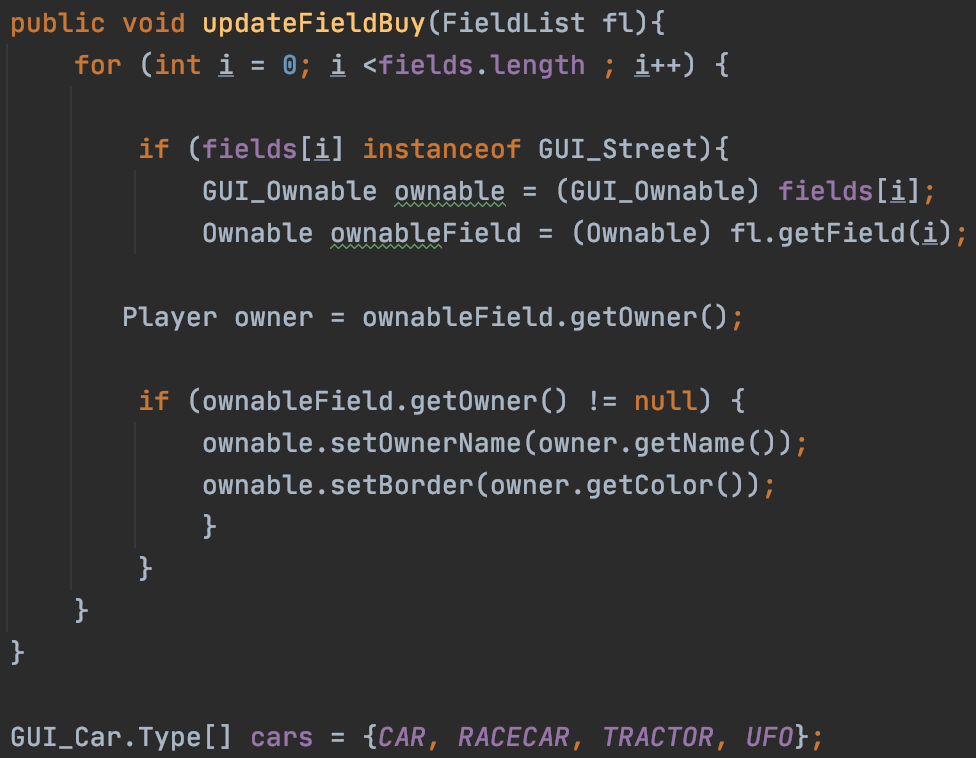
\includegraphics{sources/7_implementering/GameGUIupdateFieldBuy.png}
    \caption{Ejer af felter}
    \label{fig:GUIfeltEjer}
\end{figure}
